\documentclass[a4paper,12pt]{article} 

%%% Работа с русским языком
\usepackage{cmap}                           % поиск в PDF
\usepackage{mathtext} 			 	       % русские буквы в формулах
\usepackage[T2A]{fontenc}               % кодировка
\usepackage[utf8]{inputenc}              % кодировка исходного текста
\usepackage[english,russian]{babel}  % локализация и переносы

%Матеша
\usepackage{amsmath,amsfonts,amssymb,amsthm,mathtools} % AMS
\usepackage{icomma} % "Умная" запятая
\usepackage{float}

%\mathtoolsset{showonlyrefs=true} % Показывать номера только у тех формул, на которые есть \eqref{} в тексте.

%% Шрифты
\usepackage{euscript}	 % Шрифт Евклид
\usepackage{mathrsfs} % Красивый матшрифт
\usepackage{array}

\newcolumntype{C}[1]{>{\centering\arraybackslash}p{#1}}

%% Свои команды
\DeclareMathOperator{\sgn}{\mathop{sgn}}

%% Перенос знаков в формулах (по Львовскому)
\newcommand*{\hm}[1]{#1\nobreak\discretionary{}
{\hbox{$\mathsurround=0pt #1$}}{}}

\usepackage{geometry}
 \geometry{
 a4paper,
 top=25mm,
 }





\usepackage{graphicx}
\usepackage{amsmath,amsfonts,amssymb,amsthm,mathtools} % AMS
\usepackage{icomma} % "Умная" запятая

%\mathtoolsset{showonlyrefs=true} % Показывать номера только у тех формул, на которые есть \eqref{} в тексте.

%% Шрифты
\usepackage{euscript}	 % Шрифт Евклид
\usepackage{mathrsfs} % Красивый матшрифт
\begin{document}
    \begin{titlepage}
    \begin{center}
        \vspace{4cm}
        \huge {\textbf{Отчет о выполнении лабораторной работы 1.2.3}} \\
        \vspace{1cm}
        \Large {\textbf{Определение моментов инерции твёрдых тел}} \\
        \Large {\textbf{с помощью трифилярного подвеса}} \\
        \vspace{10cm}
        \begin{flushright}
        \begin{minipage}{.45\textwidth}
        \normalsize{\textbf{Студент:} Копытова Виктория Сергеевна}\\
        \textbf{Группа:} Б03-304\\
        \end{minipage}
        \end{flushright}   
    \end{center}
    \end{titlepage}
\newpage
 
\section{Аннотация}
\paragraph{}\textbf{Цель работы:} измерение момента инерции ряда тел и сравнение результатов с расчетами по теоретическим формулам; проверка аддитивности моментов инерции и справедливости формулы Гюйгенса-Штейнера.
	
\textbf{В работе используются:} трифилярный подвес, секундомер, счетчик числа колебаний, набор тел, момент инерции которых надлежит измерить (диск, стержень, полый цилиндр и другие).

\section{Теоретические сведения}
\paragraph{}Момент инерции твердого тела относительно неподвижной оси вращения вычисляется по формуле
\begin{equation}
    I = \int r^2 dm.
\end{equation}
Здесь $r$ - расстояние элемента массы тела $dm$ от оси вращения. Интегрирование проводится по всей массе тела m.

Для экспериментального определения момента инерции удобно использовать устройство, показанное на рис. 1 и называемое трифилярным подвесом. Оно состоит из укрепленной на некоторой высоте неподвижной платформы $Р$ и подвешенной к ней на трех симметрично расположенных нитях $АА'$, $BB'$ и $СС'$ вращающейся платформы $Р'$.
Платформа $Р$ укреплена на кронштейне и снабжена рычагом (на рисунке не показан), при помощи которого в системе можно создать крутильные колебания путем небольшого поворота верхней платформы. После того, как нижняя платформа $Р"$ оказывается повернутой на угол $\varphi$ отпосительно верхней платформы $Р$, возникает момент сил, стремящийся вернуть нижнюю платформу в положение равновесия, при котором относительный поворот платформ отсутствует. Но в положении равновесия платформа не останавливается, так как имеет угловую скорость (кинетическую энергию вращения). В результате платформа совершает крутильные колебания.
\begin{figure}
    \centering
    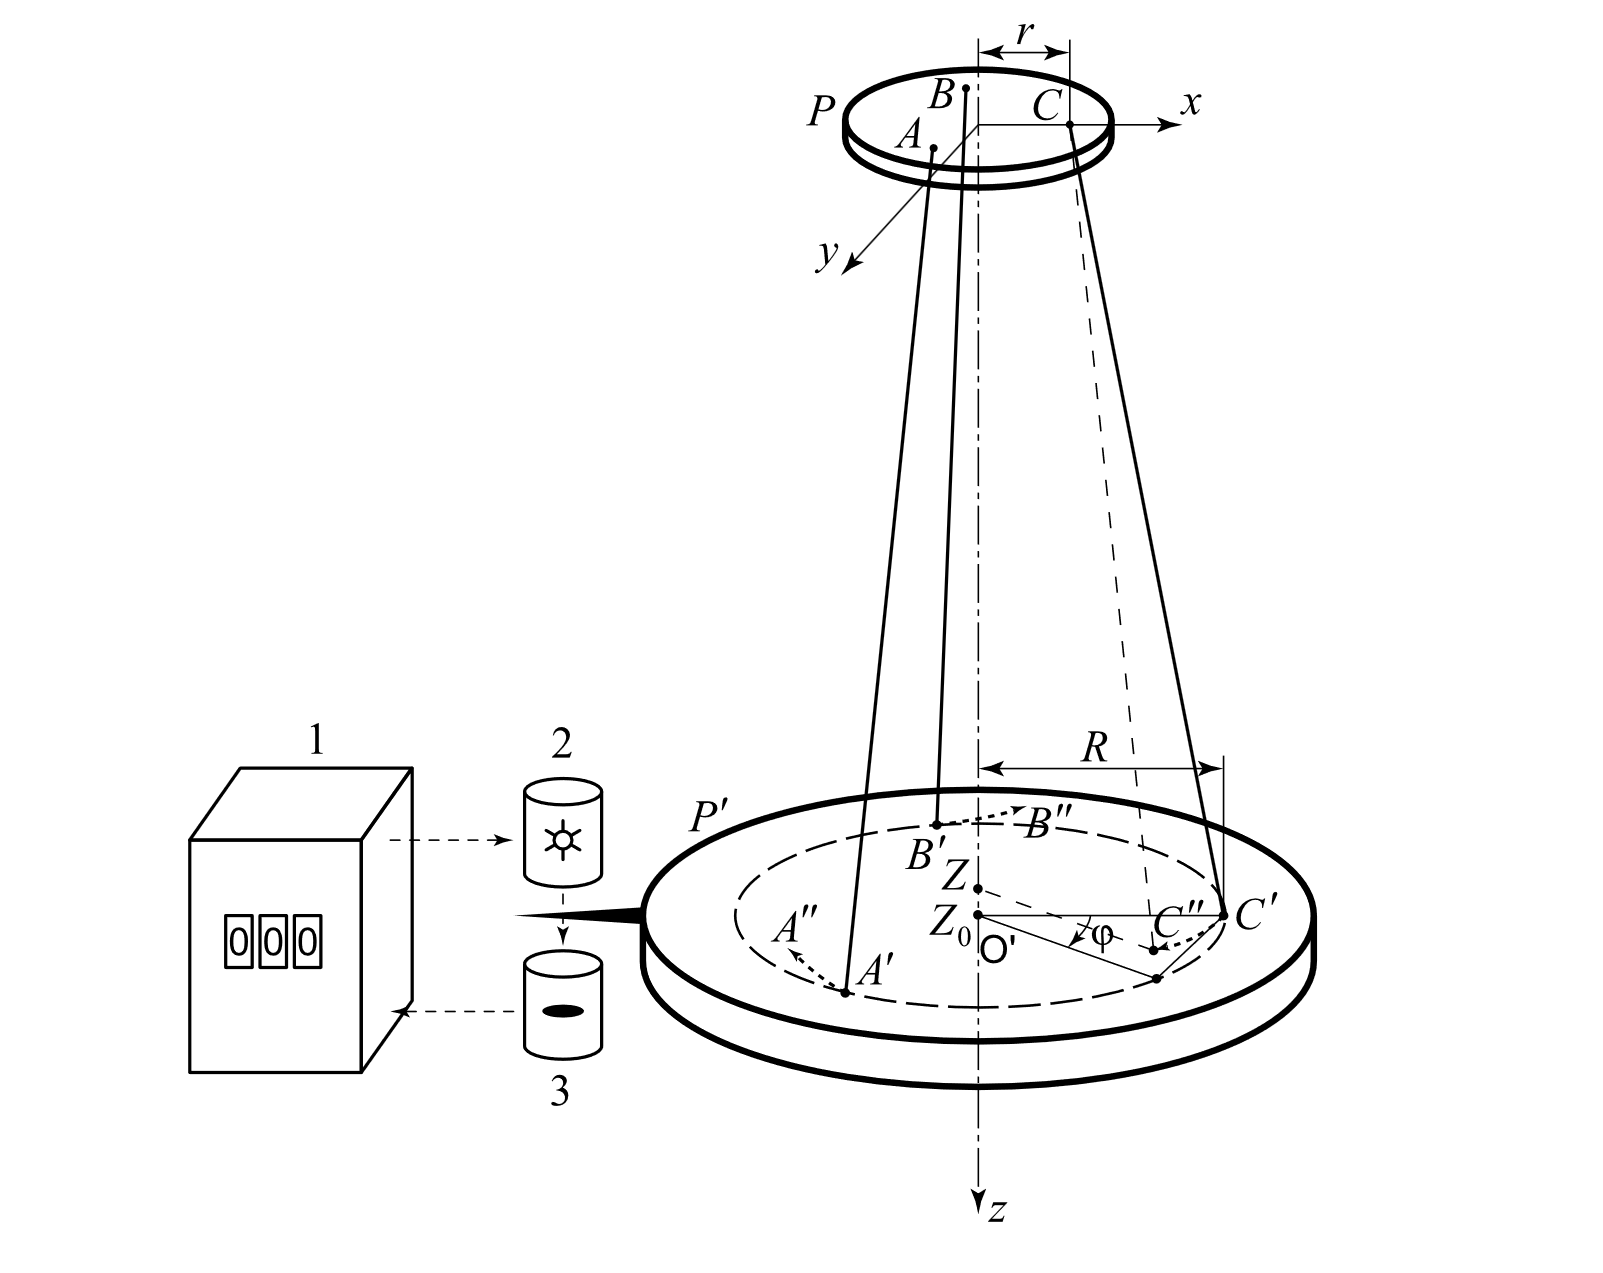
\includegraphics[scale = 0.4]{подвес.png}
    \caption{Трифилярный подвес}
\end{figure}

Если пренебречь потерями энергии на трение (о воздух и в креплениях нитей), то уравнение сохранения энергии при колебаниях можно записать следующим образом:
\begin{equation}
    \frac{I \dot \varphi^2}{2} + mg(z_0 - z) = E.
\end{equation}
Здесь $I$ -- момент инерции платформы вместе с исследуемым телом, $m$ -- масса платформы с телом, $\varphi$ -- угол поворота платформы от положения равновесия системы, точкой обозначена производная по времени (угловая скорость), $z_0$ - координата по вертикали центра нижней платформы $O'$ при равновесии ($\varphi=0$), $z$ - координата той же точки при некотором угле поворота $\varphi$. Первый член в левой части уравнения -- кинетическая энергия вращения, второй член -- потенциальная энергия в поле тяжести, $E$ - полная энергия системы (платформы с телом).

Как показывает соотношение (2), возвращающая сила возникает благодаря силе тяжести.

Воспользуемся системой координат $х, у, z$, связанной с верхней платформой, как показано на рис. 1. Координаты верхнего конца одной из нитей подвеса точки $С$ в этой системе -- ($r$, 0, 0). Нижний конец данной нити $С'$, находящийся на нижней платформе, при равновесии имеет координаты ($R$, 0, $z_0$), а при повороте платформы на угол $\varphi$ эта точка переходит в $C"$ с координатами ($R \cos \varphi, R \sin \varphi, z$). Расстояние между точками $С$ и $С"$ равно длине нити $L$. Поэтому
\begin{equation}
    (R \cos \varphi - r)^2 + R^2 \sin^2 \varphi + z^2 = L^2.
\end{equation}
Учитывая, что при малых углах поворота $\cos \varphi \approx 1 - \varphi^2/2$, получаем
\begin{equation}
    z^2 \approx z_0 ^2 - Rr \varphi^2.
\end{equation}
Извлекая из (4) квадратный корень и учитывая малость угла $\varphi$, имеем
\begin{equation}
    z \approx z_0 - \frac{Rr \varphi^2}{2z_0}
\end{equation}
Подставляя это значение $z$ в уравнение (2), получаем
\begin{equation}
    \frac{1}{2} I \dot\varphi^2 + mg \frac{Rr}{2z_0} \varphi^2 = E.
\end{equation}

Дифференцируя по времени и сокращая на $\dot\varphi$, находим уравнение крутильных колебаний системы:
\begin{equation}
    I \ddot\varphi + mg \frac{Rr}{z_0} \varphi = 0.
\end{equation}
Производная по времени от Е равна нулю, так как потерями энергии на трение пренебрегаем. Решение этого уравнения имеет вид
\begin{equation}
    \varphi = \varphi_0 \bigg ( \sqrt{\frac{mgRr}{Iz_0} t } + \theta \bigg ).
\end{equation}
Здесь амплитуда $\varphi_0$ и фаза $\theta$ колебаний определяются начальными условиями. Период крутильных колебаний системы равен
\begin{equation}
    T = 2 \pi \sqrt{\frac{Iz_0}{mgRr}}.
\end{equation}
Из (9) находим формулу для определения момента инерции:
\begin{equation}
    I = \frac{mgRrT^2}{4\pi^2 z_0}.
\end{equation}

Учитывая, что параметры установки $R$, $r$ и $z_0$ при проведении опытов не меняются, удобно переписать последнее уравнение следующим образом:
\begin{equation}
    I = kmT^2.
\end{equation}
Здесь 
\begin{displaymath}
    k = \frac{gRr}{4\pi^2 z_0}
\end{displaymath}
-- величина, постоянная для каждой установки.


\section{Ход работы}
Характеристики трифилярного подвеса:
\begin{displaymath}
    z_0 = 2.155 \pm 0.001 \quad м, 
\end{displaymath}
\begin{displaymath}
    R = (115.5 \pm 0.5) \quad мм,
\end{displaymath}
\begin{displaymath}
    r = (30.2 \pm 0.3) \quad мм,
\end{displaymath}
\begin{displaymath}
    m =(1026.4 \pm 0.5) \quad г,
\end{displaymath}
\begin{displaymath}
    k = \frac{gRr}{4\pi^2 z_0}
\end{displaymath}
\begin{displaymath}
    \sigma_k = k  \sqrt{\left( \dfrac{\sigma_R}{R}\right)^2 + \left( \dfrac{\sigma_r}{r}\right)^2 + \left( \dfrac{\sigma_{z_0}}{z_0}\right)^2}
\end{displaymath}
\begin{displaymath}
    k = (4.02\pm 0.04) \cdot 10^{-4} \quad м^2/с^2
\end{displaymath}

Параметры тел: диаметр диска -- $16.5 \pm 0.05$ см, диаметр кольца -- $14.9 \pm 0.05$ см, длина бруска -- $a = (20.9 \pm 0.05)$ cм, высота бруска -- $b = (2.9 \pm 0.05) см$.
\begin{enumerate}
    \item Будем измерять период колебаний платформы с различными грузами. Результаты занесём в таблицу 1.
    \begin{table}[H]
        \centering
        \begin{tabular}{|C{1.2 cm}|C{2 cm}|C{2 cm}|C{2 cm}|C{2 cm}|C{2 cm}|}
            \hline
            № опыта& $T$ платформы, с & $T$ платформы и диска, с & $T$ платформы и кольца, с & $T$ платфомы и бруска, с & $T$ платорфмы, кольца и диска, с \\
            \hline
            1 & 4.421 & 3.974 & 4.205 & 3.782 & 3.941 \\
            \hline
            2 & 4.429 & 3.960 & 4.200 & 3.900 & 3.949 \\
            \hline
            3 & 4.412 & 3.964 & 4.196 & 3.772 & 3.932 \\
            \hline
            4 & 4.422 & 3.964 & 4.211  & 3.758  & 3.947 \\
            \hline
            5 & 4.426 & 3.960 & 4.218  & 3.746 & 3.939\\
            \hline 
            
        \end{tabular}
        \caption{Периоды колебаний платформы с различными грузами}
    \end{table} 
    
    Рассчитаем моменты инерции тел по формуле (11).

    Погрешность измернения момента инерции:
    \begin{displaymath}
        \varepsilon_I = I \sqrt{\left( \dfrac{\sigma_k}{k} \right)^2 + \left( \dfrac{\sigma_m}{m}\right)^2 + 2 \left( \dfrac{\sigma_T}{T}\right)^2} \approx 0.01
    \end{displaymath}
    
    \begin{table}[H]
        \centering
        \begin{tabular}{|C{3 cm}|c|c|C{2 cm}|}
            \hline
             Тело & Масса, г & Период, c & Момент инерции, $г \cdot м^2$ \\ 
             \hline
             Платформа & 1026.4 & 4.422 & $8.07 \pm 0.08$ \\
             \hline
             Платформа и диск & 1610.8 & 3.964 & $10.18 \pm 0.1$ \\
             \hline
             Платформа и кольцо & 1757.1 & 4.206 & $12.50 \pm 0.13$ \\
             \hline
             Платформа и брусок & 2226.4 & 3.792 & $12.87 \pm 0.13$ \\
             \hline
             Платформа, диск и кольцо & 2341.5 & 3.942 & $14.63 \pm 0.15$ \\
             \hline
        \end{tabular}
        \caption{Моменты инерции тел}
    \end{table}

    Можно увидеть, что сумма момента инерции платформы и кольца и разности момента инерции платформы и диска и платформы $12.5 + (10.18-8.07) = 14.61 \approx 14.63$ -- момент инерции платформы, диска и кольца с погрешностью 1\%, что доказывает аддитивность моментов инерции.

    

    Сравним полученные значения с теоретическими.
    \begin{table}[H]
        \centering
        \begin{tabular}{|C{3 cm}|C{3 cm}|C{3 cm}|C{3 cm}|}
            \hline
            & & & \\
            Тело & Теор. формула $I$ & Теор. значение $I$, $г \cdot м^2$ & Измеренное значение $I$, $г \cdot м^2$ \\
            \hline
            & & & \\
            Диск & $\frac{1}{2} mr^2$ & $1.99 \pm 0.02$ & $2.11 \pm 0.18$  \\
            & & & \\
            \hline
            & & & \\
            Кольцо & $mr^2$ & $4.05 \pm 0.04$ & $3.8 \pm 0.21$ \\
            & & & \\
            \hline
            & & & \\
            Брусок & $\frac{1}{12} m(a^2+b^2)$ & $4.46 \pm 0.04 $ & $4.74 \pm 0.21$ \\
            & & & \\
            \hline
        \end{tabular}
        \caption{Сравнение экспериментальных и теоретических значений моментов инерции}
    \end{table}

    Экспериментальные данные соответствуют теоретическим в пределах погрешности.
    \item Поместим на платформу диск, разрезанный по диаметру. будем постепенно раздвигать половинки диска так, чтобы их общий центр масс всё время оставался на оси вращения платформы (рисунок 2). Снимем зависимость момента инерции такой системы $I$ от расстояние $h$ каждой из половинок до оси вращения (центра платформы).
    \begin{figure}[H]
        \centering
        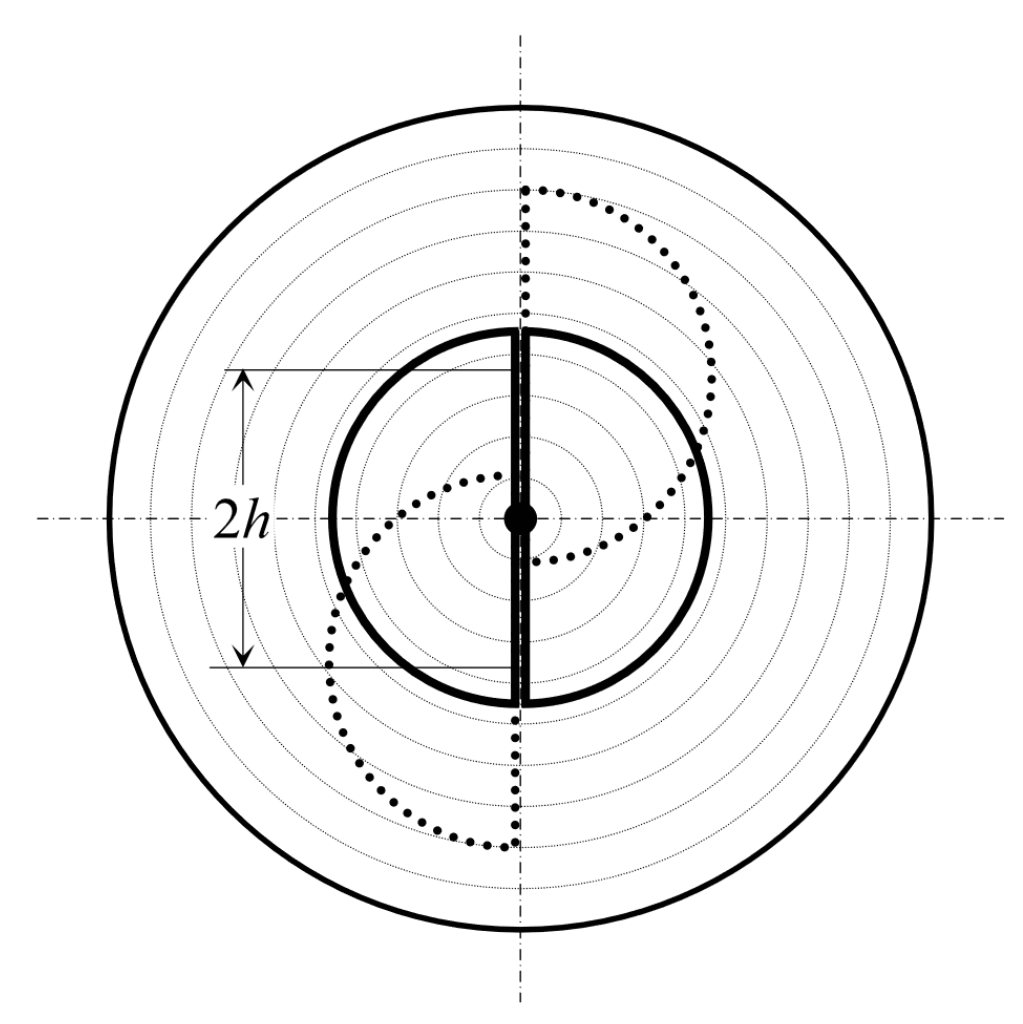
\includegraphics[scale = 0.3]{h.png}
        \caption{Расположение тел на платформе}
    \end{figure}

    Построим график зависимости $I(h)$ и определим по нему массу и момент инерции диска.
    \begin{table}[H]
        \centering
        \begin{tabular}{|C{3 cm}|C{2 cm}|C{2 cm}|C{2 cm}|}
            \hline
            Cреднее значение периода $T$, c & h, см & $I, г \cdot м^2$ & $\sigma_I$, $кг \cdot м^2$ \\
            \hline
             3.094 & 0   & 9.83  & 0.10 \\
             \hline
             3.111 & 1   & 9.94  & 0.10 \\
             \hline
             3.166 & 2   & 10.29 &  0.10 \\
             \hline
             3.238 & 2.5 & 10.77 & 0.11 \\
             \hline
             3.302 & 3   & 11.20 & 0.11 \\
             \hline
             3.445 & 4   & 12.19 & 0.12 \\
             \hline
             3.544 & 4.5 & 12.90 & 0.13 \\
             \hline
             3.865 & 6   & 15.34 & 0.15 \\
             \hline
        \end{tabular}
        \caption{Моменты инерции системы в зависимости от $h$}
    \end{table}

    Построим график зависимости $I(h^2)$:
    \begin{figure}[H]
        \centering
        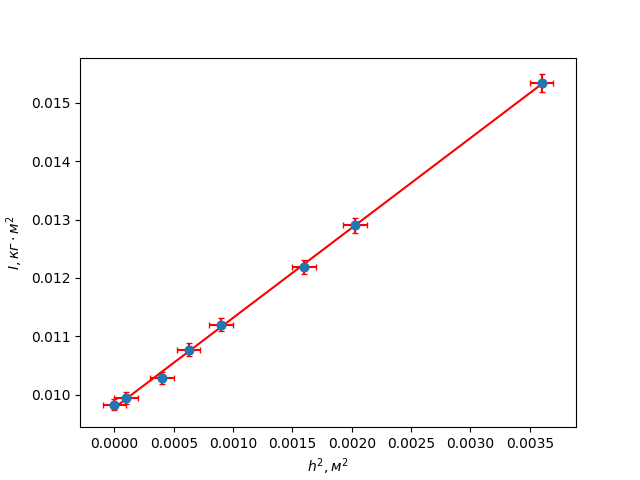
\includegraphics[scale = 0.8]{1.png}
        \caption{Зависимость $I(h^2)$}
    \end{figure}

    Мы видим, что зависимость линейная, значит
    \begin{displaymath}
        I = I_0 + bh^2,
    \end{displaymath}
    где $I_0$ -- момент инерции диска и платформы, $b$ -- масса диска.
    По методу наименьших квадратов:
    \begin{displaymath}
        I_0 = (9.78 \pm 0.1) \quad г \cdot м^2,
    \end{displaymath}
    \begin{displaymath}
        b = (1.541 \pm 0.01)\quad кг,
    \end{displaymath}
    \begin{displaymath}
        I_{диска} = (1.71 \pm 0.18) \quad г \cdot м^2.
    \end{displaymath}
    Теоретические значения: $b = (1528 \pm 1) \quad г$, $I_{диска} = 1.56 \quad г \cdot м^2$.
    
    Теоретические значения совпадают с экспериментальными в пределах погрешности.

\end{enumerate}
	
\section{Вывод} 

\paragraph{}В ходе работы были измеряны моменты инерции различных тел с дочтаточно высокой точностью в $5.5 \%$. Полученные значения достаточно точно сходятся с теоретическими, что позволяет говорить о достоверности использованного метода измерения.

Была доказана аддитивность момента инерции и с помощью трифилярного подвеса была определена масса исследуемого тела и его момента инерции из зависимости полного момента инерции и платформы от расстояние от тела до оси вращения.

\end{document}


